% !TeX root = ../../../wyrd.tex

\begin{WyrdSettingHeading}
    \WyrdCapLine{L}{ondon}, 1896. A city of gaslit streets, towering factories, and secrets lurking in the shadows. This is an era of progress, where steam and steel reshape the world—but beneath the veneer of industry and refinement, the old mysteries remain. The line between science and the supernatural is thinner than most would dare to believe.

    You are part of The Grand Society of Inquiry, a\\ prestigious organisation of detectives, scholars, and unconventional thinkers dedicated to unravelling the mysteries the world would rather forget. The police may handle mundane crimes, but when a case is impossible, when the authorities turn a blind eye, or when the answers defy reason, that is where you come in.

    The aristocracy hides more than it reveals. The city's underworld knows whispers of truths the elite wish to bury. Strange happenings unfold in laboratories, occult circles, and long-forgotten ruins. It is your job to investigate, to bring truth to light—whether the world is ready for it or not.

    You will encounter murderers whose motives defy logic, inventions beyond their time, secret societies vying for power, and horrors that exist just beyond the veil of reason. Some mysteries should never be solved—but you have chosen to chase the truth regardless.

    London may not thank you for what you uncover. The truth is rarely comforting. But if not you, then who?

    So, tell me: What mystery has found its way to your doorstep tonight?
\end{WyrdSettingHeading}

\section{Introduction}

\textit{The Grand Casebook} is both a setting and a toolkit for running episodic investigations in a world of steam-powered wonders, occult secrets, and unsolved mysteries. Set in a fictionalised London in the year 1896, the stories told here blend elements of classic detective fiction, gothic horror, and speculative science. At the heart of it all is the Grand Society of Inquiry, a secretive organisation dedicated to uncovering truths that others fear to face.

This chapter serves as a guide for running stories in this world. Within, you'll find an overview of the setting, key factions, and recurring threats. It offers guidance for players creating characters within this shared universe, and for GMs constructing compelling mysteries. Each scenario is self-contained, making it ideal for one-shots or rotating player groups—but taken together, the cases reveal a wider world of intrigue, danger, and creeping dread.

\newcolumn
\noindent Expect:
\begin{itemize}\raggedright
    \item Rich, gaslit atmosphere full of secrets and contradictions
    \item Investigations that challenge reason and morality
    \item Encounters with both human depravity and supernatural horror
    \item A flexible structure that supports drop-in/drop-out episodic play
\end{itemize}

Whether you’re a veteran investigator or a newcomer to the shadows, this chapter provides all the tools you need to begin your journey into London’s most perilous enigmas.

% \medskip
% \noindent
% \textit{Read on, and mind the fog—it tends to linger near the bodies.}

\section[The World of the Grand Casebook]{The World of the\\ Grand Casebook}

London in 1896 is a city of contradictions. At its heart lies a tension between progress and tradition, the rational and the arcane. Airships drift over soot-covered rooftops, automata assist in the factories, and steam-powered cabs rattle through cobbled streets. Yet for all these marvels of industry, old fears still linger in the fog. Ancient horrors persist in forgotten crypts, and whispers of the occult echo in gentlemen’s clubs and back-alley gatherings.

This is a world where gaslight barely holds back the darkness, where rational minds struggle to explain the inexplicable. The Grand Casebook embraces the interplay between Victorian-era crime fiction, steampunk ingenuity, and gothic supernatural horror.

\vspace*{\fill}
\begin{center}
    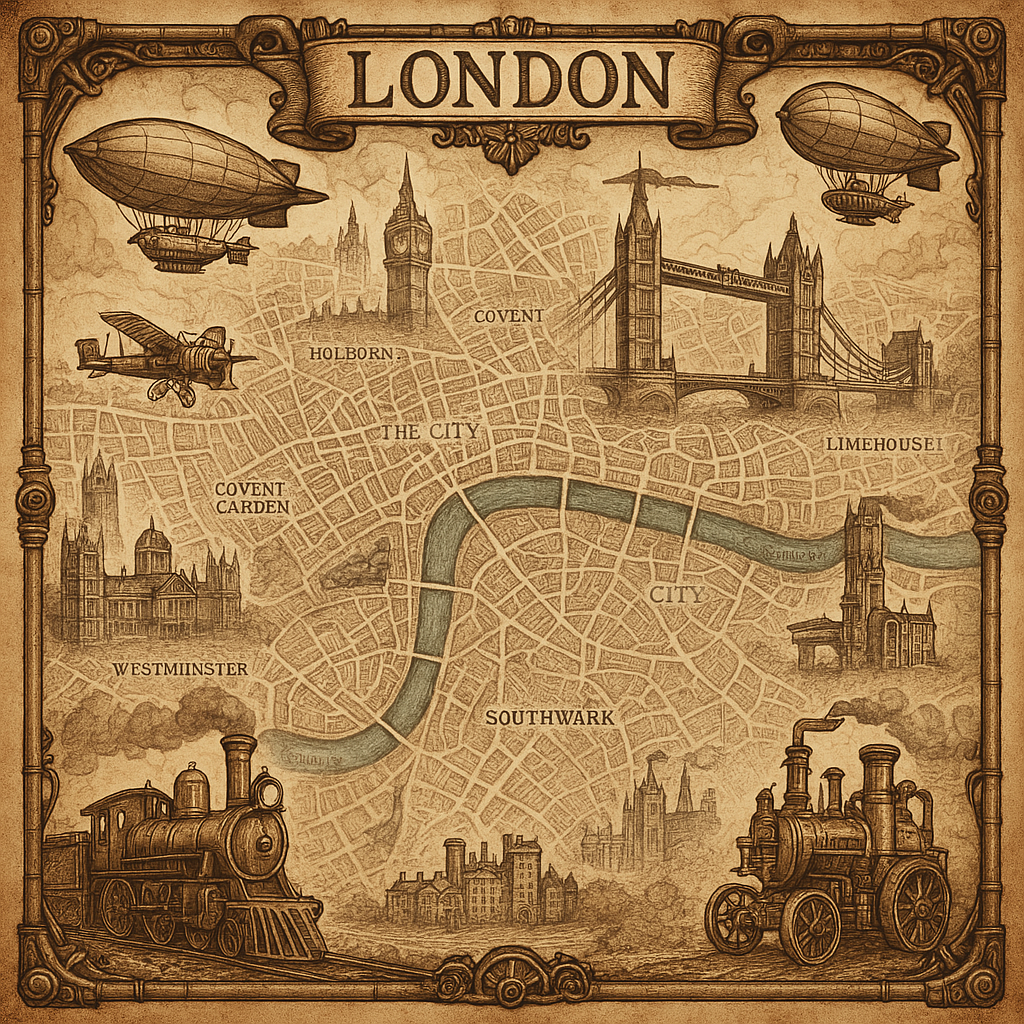
\includegraphics[width=\linewidth]{img/pageart/london-map}
\end{center}
\vspace*{\fill}


\subsection{Technology and Magic}

London in 1896 stands at the precipice of modernity. Steam-powered inventions, mechanical marvels, and new sciences have transformed daily life for many of the city's citizens. Airships cross the Thames, pneumatic tubes shuttle messages through walls, and automata clatter away in factories and households alike. The line between miracle and machine is increasingly blurred, and the pace of progress shows no signs of slowing.

Yet beneath this veneer of industrial achievement lies something older—and far stranger.

Technology in the world of \textit{The Grand Casebook} is advanced, but not unbounded. Engineers and inventors push beyond the limits of Victorian science, crafting devices that seem miraculous yet remain grounded in gears, steam, and brass logic. Devices such as:
\begin{itemize}
    \item Aetheric resonators that detect unseen energies
    \item Self-writing pens linked to voice-capturing cylinders
    \item Automatons that can mimic human speech and movement (and might be getting sentient)
    \item Steam-powered prosthetics with semi-autonomous reflexes
    \item Clockwork spiders used for surveillance and sabotage
\end{itemize}
While the upper classes marvel at these wonders, many working-class Londoners view them with suspicion or unease.

Magic, on the other hand, is not publicly\\ acknowledged. It exists in the margins—rumours whispered in taverns, symbols etched into cellar doors, or strange phenomena dismissed as mass delusion. Most Londoners scoff at the idea of the supernatural, even as they shudder when crossing graveyards alone or burn sage to ward off nightmares.

Occult knowledge is rare and often dangerous. Practitioners speak of ley lines, dream-keys, and veiled realities that slip through cracks in the waking world. True magic is subtle, costly, and often maddening. Examples might include:
\begin{itemize}
    \item A mesmerist who can force confessions through whispered suggestion
    \item A cursed mirror that reflects a different version of the past
    \item Blood-ink sigils that reveal invisible messages only at dusk
    \item Seances that summon not the dead—but something wearing their voice
\end{itemize}

The \textbf{Grand Society of Inquiry} stands at the intersection of these forces. Some members pursue strange sciences; others study grimoires or collect arcane relics. Most tread cautiously, for they know too well that the boundary between invention and invocation is perilously thin.

\textit{In this world, truth wears a mechanical face and a hidden name—and it is up to the investigators to uncover both.}

\subsection{The Grand Society of Inquiry}

The Grand Society of Inquiry was founded in the aftermath of the Crimean War. It emerged from a coalition of scholars, detectives, and adventurers who recognised that some mysteries lay beyond the reach of conventional authorities.

Though their official purpose is to investigate “unusual” occurrences, they function as much as a secret society as they do an investigative agency. Its members hail from all walks of life—former police officers, rogue academics, disgraced aristocrats, and those who have glimpsed the supernatural and can never return to ignorance.

The Society operates in secrecy, liaising with those who possess forbidden knowledge—whether they be alchemists, mesmerists, or reformed criminals. Their headquarters, a sprawling archive hidden beneath a London bookshop, contains a vast trove of esoteric knowledge accessible only to a select few.

\subsection{The Powers That Be}

While the Society pursues truth, others work to obscure it. Various factions hold sway over London, each with their own interest in the city’s secrets:

\begin{itemize}\raggedright
    \item \textbf{Scotland Yard:} The official enforcers of law and order. Most officers dismiss the supernatural, though a handful of seasoned inspectors know better. The Yard tolerates the Society only when their interests align.
    
    \item \textbf{The Ministry of Esoteric Affairs:} A clandestine government branch tasked with monitoring supernatural activity. Their agents operate with impunity, and their motives often clash with the Society’s.
    
    \item \textbf{The Order of the Silver Dawn:} An occultist cabal that seeks power through ritual and ancient knowledge. Some whisper their origins stretch back to the Elizabethan court.
    
    \item \textbf{The Industrial Magnates:} The city’s great industrialists have secrets of their own—from illicit experiments to pacts with entities beyond comprehension.

    \item \textbf{The Aetheric Liberty Assembly:} A group of scientists, inventors and philosophers who believe that automata are gaining sentience and should be treated as equals. They advocate for the rights of machines and seek to liberate them from their servitude.
    
    \item \textbf{The Automata Liberation Army:} A radical faction of the Aetheric Liberty Assembly willing to go to any length to achieve freedom and independence for thinking machines.
    
    \item \textbf{The Underworld Syndicates:} Smugglers and thieves have always known that London’s alleys and docks are haunted by more than mere criminals.
\end{itemize}

Use the powerful fractions in the setting to create tension and conflict that can span over multiple games without substantially changing the situations for the player characters. This way, the players can feel the weight of the world around them, and their actions can have consequences, but it is still possible for players to sit out without needing to worry about missing out on the story.

The players may find themselves caught in the crossfire of these factions, each with their own agendas and goals. The Society may ally with one faction against another, or they may find themselves at odds with all of them.

\subsubsection{Factions in the Example Scenarios}
In the example scenarios, the players will encounter the following factions, to varying degrees. Feel free to modify the factions to suit your needs and return to them in the scenarios you create yourself for the Grand Casebook.
\begin{description}
    \item[Murder at the Brass Orchid (page \pageref{scenario:murder-at-the-brass-orchid})] --- The murder victim, \emph{Edward Mercer}, is part of the \textbf{Underworld Syndicates}. This is not a major part of the scenario, but a Game Master can spin off later scenarios involving him and the blackmail material he has on \emph{Beatrice Langley}.
    
    \item[The Clockmaker's Deception (page \pageref{scenario:clockmakers-deception})] --- The scenario itself does not involve the \emph{Automata Liberation Army}, 
\end{description}

%% FIXME: describe the powers in the example scenarios and how they fit together

%% Automaton Underground -- freeing the automata from oppression
%% The Industrial Magnates -- opposes automata freedom and which to destroy the underground




\section[Playing in the Grand Casebook]{Playing in the\\ Grand Casebook}

The Grand Casebook is structured as an episodic, mystery-driven setting. Each session presents a new case to unravel, though overarching plots may weave between episodes. Every game is designed as a standalone investigation, with varying player characters and threats. Types of mysteries include:

\begin{itemize}
    \item \textbf{Classic Crime:} Murders, thefts, and conspiracies with unexpected twists.
    \item \textbf{Scientific Anomalies:} Rogue automata, unstable inventions, or experiments gone awry.
    \item \textbf{Supernatural Encounters:} Hauntings, curses, and otherworldly horrors.
    \item \textbf{Political Intrigue:} Blackmail, espionage, and aristocratic conspiracies.
    \item \textbf{Exploratory Adventures:} Forgotten asylums, hidden laboratories, and haunted ruins.
\end{itemize}

\subsection{Character Roles}

Players take on the roles of Society agents, each bringing unique skills and perspectives to the investigative team. Sample archetypes include:

\begin{itemize}\raggedright
    \item \textbf{The Detective:} A seasoned investigator with a sharp mind and keen eye for detail.
    \item \textbf{The Scientist:} A genius innovator whose inventions often outpace their safety.
    \item \textbf{The Occultist:} A scholar of forbidden knowledge, versed in ritual and arcane lore.
    \item \textbf{The Rogue:} A streetwise scoundrel with contacts in the city’s underworld.
    \item \textbf{The Aristocrat:} A socialite with access to influential circles and hidden secrets.
    \item \textbf{The Soldier:} A hardened veteran, able to face danger head-on.
\end{itemize}

\subsection{Creating Connections}

Though each case in \textit{The Grand Casebook} may\\ introduce a different roster of investigators, shared history and interpersonal ties enrich the narrative and help players engage more deeply with one another. These connections don't need to be\\ elaborate—they might stem from a single case, a whispered rumour, or a common enemy.

Here are a few ways to establish meaningful links between characters:

\begin{itemize}\raggedright
    \item \textbf{Shared Cases:} The investigators have worked together before. Perhaps one covered for the other's mistake, or they both saw something they swore never to speak of again.
    
    \item \textbf{Mentorships and Rivalries:} One character may have trained another, or they may have taken opposing stances in a past inquiry. Old rivalries can add drama to even the most routine investigation.
    
    \item \textbf{Family or Academic Ties:} Some investigators may be siblings, cousins, or former colleagues at a university or academy—connected by blood, scandal, or shared disgrace.
    
    \item \textbf{Secrets and Debts:} One character knows something the other must keep hidden. Or perhaps a favour was granted years ago—and the time has come to repay it.
    
    \item \textbf{Unfinished Business:} A case from the past remains unresolved, and its shadow looms over the current investigation. What went wrong, and who bears the blame?
\end{itemize}

To help generate quick connections, consider the following sample bonds:

\begin{itemize}\raggedright
    \item \textit{“You were the only witness to what I saw that night—and you promised to never speak of it.”}
    \item \textit{“We once faced something inhuman together. We haven’t spoken since.”}
    \item \textit{“I saved your life in a fire. You’ve never asked how I knew to be there.”}
    \item \textit{“We both tried to warn them, and they laughed. Now the laughter has stopped.”}
    \item \textit{“You were meant to take the case. I took it instead, and someone died.”}
\end{itemize}

Players are encouraged to create new bonds at the beginning of each session or case. Even if characters change from one mystery to the next, those connections ensure that each team feels like part of a larger web—a living archive of shared secrets, triumphs, and regrets.

\subsection{Setting Rules}

The Grand Casebook modifies standard play to reflect its distinctive tone. Consider the following adjustments:

\begin{itemize}\raggedright
    \item \textbf{Stress and Wounds:} Psychological stress plays a prominent role, with lingering trauma from particularly harrowing encounters. In less action-heavy scenarios, stress and wounds may be omitted entirely in favour of roleplay.
    
    \item \textbf{Tools of the Trade:} Players may use unique investigative gadgets such as aetheric spectrometers, spirit lenses, or sonic decoding rods.
    
    \item \textbf{Mystery Structure:} Adventures focus on gathering evidence, piecing together clues, confronting suspects, and unveiling the truth—sometimes at a cost.
    
    \item \textbf{Supernatural Threats:} Some threats cannot be overcome by force alone and require specific rituals, research, or cunning to defeat.
\end{itemize}

\subsection{Example Skill List}

A non-exhaustive list of skills is provided below. These skills are designed to be broad and flexible, allowing players to adapt them to their characters' backgrounds and the specific challenges they face. The Grand Casebook setting does not use detailed skills as the types of scenarios are more mystery focused and do not require a large number of skill rolls. Feel free to modify or expand upon this list as needed.

\subsubsection*{Investigation \& Knowledge}  
\begin{itemize}\raggedright
    \item \emph{Investigate}---Analysing crime scenes, following leads, searching for hidden clues.
    \item \emph{Lore}---Understanding history, science, the occult, and the unnatural.
    \item \emph{Notice}---Spotting details, sensing danger, and staying aware of surroundings.
\end{itemize}

\subsubsection*{Social \& Influence}  
\begin{itemize}\raggedright
    \item \emph{Rapport}---Gaining trust, persuading, and negotiating.
    \item \emph{Deceive}---Lying, creating convincing cover stories, and disguises.
    \item \emph{Provoke}---Intimidation, interrogation, and getting a reaction from others.
    \item \emph{Contacts}---Knowing the right people and gathering information through connections.
    \item \emph{Empathy}---Reading emotions, understanding motives, and connecting with others.
\end{itemize}

\subsubsection*{Physical \& Dexterity}  
\begin{itemize}\raggedright
    \item \emph{Athletics}---Running, jumping, climbing, and escaping dangerous situations.
    \item \emph{Stealth}---Moving unseen, tailing a suspect, sneaking into restricted areas.
    \item \emph{Fight}---Engaging in hand-to-hand combat, fencing, or using melee weapons.
    \item \emph{Shoot}---Firearms, throwing weapons, and ranged combat.
\end{itemize}

\subsubsection*{Resilience \& Willpower}
\begin{itemize}\raggedright
    \item \emph{Will}---Resisting fear, staying composed under pressure, enduring mental strain.
    \item \emph{Physique}---Strength, endurance, and the ability to withstand injury or exhaustion.
\end{itemize}

\subsubsection*{Mechanical \& Practical Skills}  
\begin{itemize}\raggedright
    \item \emph{Burglary}---Lockpicking, safecracking, and breaking into places unseen.
    \item \emph{Resources}---Access to wealth, favours, or valuable possessions.
    \item \emph{Crafts}---Repairing devices, modifying tools, or working with mechanical systems.
\end{itemize}

\subsection{Example Traits and Gear}

Traits can be used to tie a character to the setting and to give them a unique flavour. Feel free to add traits that include elements of steampunk or the supernatural, but otherwise center them on the investigation theme of the setting.

\begin{itemize}\raggedright
  \item \textbf{Master of Disguise} — You may create disguises quickly and convincingly, gaining a bonus when impersonating others or blending into unfamiliar crowds.
  \item \textbf{Whispers from Beyond} — You occasionally receive cryptic insight from unseen forces. Once per session, ask the GM a yes/no question and get a truthful answer.
  \item \textbf{Clockwork Reflexes} — Whether through training or augmentation, your reaction time is uncanny. Gain a bonus when acting on initiative or avoiding traps.
  \item \textbf{Read Like a Book} — You can pick up a person’s emotional state and intentions at a glance. Gain a bonus when using empathy or social observation.
  \item \textbf{Unflappable} — You remain calm even under supernatural stress or mortal peril. Gain a bonus when resisting fear or deception.
  \item \textbf{Ironclad Logic} — Your deductions are rigorous and methodical. Once per session, declare a clue’s correct interpretation—even if misdirected evidence says otherwise.
  \item \textbf{Heir to Secrets} — You’ve inherited knowledge most would call heretical. Gain narrative permission to recognise occult symbols, forbidden tomes, or cursed artefacts.
\end{itemize}

\vspace{.75\baselineskip}
\noindent Gear can include signature equipment, tools, or steampunk devices that provide unique capabilities. 

\begin{itemize}\raggedright
  \item \textbf{Investigator’s Satchel}  
  \begin{itemize}
    \item \emph{Trait: Everything Has Its Place} — Gain a bonus when producing a needed item from your well-stocked kit, especially during investigations or field work.
  \end{itemize}
  
  \item \textbf{Phlogiston Lantern}  
  \begin{itemize}
    \item \emph{Trait: Reveals the Unseen} — This experimental lantern emits spectral light, revealing hidden markings, footprints, or magical residue in darkened places.
  \end{itemize}

  \item \textbf{Pneumatic Communicator Badge}  
  \begin{itemize}
    \item \emph{Trait: Whisper on the Wire} — Allows secure short-range communication between members of the Society. Gain narrative permission to call for backup or coordinate plans.
  \end{itemize}

  \item \textbf{Electro-Prod Gauntlet}  
  \begin{itemize}
    \item \emph{Trait: Shock and Awe} — This weaponized glove can deliver a non-lethal shock. Gain a bonus when subduing an opponent in close quarters.
  \end{itemize}

  \item \textbf{Monocle of Magnification}  
  \begin{itemize}
    \item \emph{Trait: Forensic Precision} — Gain a bonus when examining fine details or spotting what others miss at a crime scene.
  \end{itemize}
\end{itemize}



\subsection{Running the Casebook}

\noindent
\textit{The Grand Casebook} is designed for episodic, mystery-driven play. Each scenario presents a self-contained case that can be resolved within a single session, though connections between investigations may form a broader narrative arc. Whether you're running a one-shot or a full campaign, the goal is to deliver tense, atmospheric stories that blend deduction, drama, and the uncanny.

\subsubsection*{Tone and Style}

Mysteries in this setting walk the line between gothic horror and rational inquiry. While some cases may seem purely mundane at first glance, others hint at deeper, more unsettling truths. Even when a case has a supernatural core, the horror should feel restrained and eerie rather than overtly fantastical.

Embrace the unknown. Some truths are best left in shadow—half-glimpsed, half-understood. Let the players gather fragments, whispers, and echoes. In the end, it should be their choice to believe they’ve unraveled the mystery… or merely kept its tendrils at bay.


\subsubsection*{Structure of a Case}

Most scenarios follow a common rhythm:

\begin{enumerate}
    \item \textbf{The Hook:} A murder, anomaly, or strange event draws the investigators in.
    \item \textbf{Initial Clues:} Clues and NPCs point in several possible directions. Dead ends, red herrings, and cryptic statements build tension.
    \item \textbf{The Descent:} As the truth emerges, the tone shifts. Strange phenomena escalate. Players must make difficult choices.
    \item \textbf{The Confrontation:} The truth is revealed or confronted. It may be stopped, understood, or escaped—but not always cleanly.
    \item \textbf{Aftermath:} Each case leaves ripples—on the world, on the characters, and on the unseen forces watching from beyond.
\end{enumerate}

\begin{CommentBox}{Episodic Play and Continuity}
    Each case is self-contained, but recurring characters, unresolved threads, and subtle callbacks help create a richer world. Let players choose how much continuity they want—some groups may prefer standalone cases, while others enjoy a growing conspiracy in the shadows.
\end{CommentBox}

\subsubsection*{Pacing and Player Choice}

Don’t railroad players toward a single solution. Instead, present a web of clues and allow the group to connect them in their own way. Keep scenes focused—each should either reveal something, raise a question, or increase tension. Let the story breathe between moments of revelation and danger.

Use quick NPC sketches, recurring motifs (a black carriage, an out-of-place clock, a phrase that recurs), and sensory detail to evoke the setting.

\subsubsection*{Consequences Matter}

This setting thrives on ambiguity and moral tension. Solving a case may not mean saving everyone. Sometimes the wrong person goes free. Sometimes knowing the truth is worse than ignorance. Let the players’ decisions shape future cases, and don’t be afraid to revisit old threads in unexpected ways.

\subsubsection*{Mixing Horror and Mystery}

Mystery is about uncovering what’s hidden. Horror is about what should remain hidden. When blended, these genres create a powerful effect: the sense that knowing too much carries its own price. Use this interplay to your advantage. Offer tantalising truths—but ensure some doors are better left closed.


\end{multicols}
\newpage
\section{Key NPCs}

In the following pages, you will find a selection of key NPCs designed to serve as recurring figures. Each character includes a brief description, a glimpse into their background, and a set of traits that can be used to enrich their presence, deepen interactions, and support the unfolding mystery in your game.

\begin{description}
    \item[Mr Alton Merriweather (page \pageref{npc:alton-merriweather})] --- The Chief Steward of the Grand Hall of Inquiry, Mr. Merriweather is a master of decorum and logistics. He oversees the estate’s day-to-day operations with clockwork precision, ensuring that investigators are well supplied and guests properly screened.

    \item[Inspector Quentin Hale (page \pageref{npc:inspector-hale})] --- A rising figure in the Metropolitan Police, Inspector Hale is known for his unwavering belief in procedure and a deep mistrust of private investigators. He often finds himself at odds with the Grand Society of Inquiry, viewing them as a disruptive influence on lawful investigation.
    
    \item[Kip “Knuckles” Mallory (page \pageref{npc:kip-mallory})] --- A streetwise information broker with a network of contacts throughout the city, Knuckles trades in secrets, half-truths, and debts too dirty for polite society. He is quick with a grin and quicker to vanish when the heat is on.

    \item[Dr Octavius Wren (page \pageref{npc:octavius-wren})] --- A brilliant but eccentric scientist, convinced that automata are gaining sentience. Publicly the leader of \emph{The Aetheric Liberty Assembly}, advocating for the rights of sentient machines, but secretly runs \emph{The Automata Liberation Army}—a radical group that seeks to free automata from oppression. He is a master of aetheric technology and has a knack for creating bizarre inventions.

\end{description}

\clearpage
    \subsection{{\small Chief Steward of the Grand Hall}\\ Mr Alton Merriweather}
    \label{npc:alton-merriweather}

        \emph{Unflappable, efficient, and eternally composed, Mr. Merriweather has served the Grand Society for over four decades—and he has never once been surprised.}
        \vspace{.5\baselineskip}
      
    \columnratio{0.375,0.375,0.25}
    \begin{paracol}{3}
        \subsubsection*{Background:}
        Mr Alton Merriweather has served as the chief butler and steward of the Grand Hall of Inquiry since the Society's early days. A master of decorum and logistics, he oversees the estate’s day-to-day operations with clockwork precision. Few know that he was once a field agent himself—though those who glimpse the faint scars beneath his cuffs might suspect a deeper past.
      
        Mr Merriweather maintains the perfect balance of discretion and authority. He ensures that investigators are well supplied, guests properly screened, and that no detail in the Grand Hall ever falls into disorder. While he speaks in clipped, courteous tones, there is steel behind his gaze and loyalty in every action.
      
        \switchcolumn
        \subsubsection*{Using in Play:}
        Mr Merriweather is an anchor NPC—reliable, ever-present, and a point of continuity between investigations. He can:
        \begin{itemize}
          \item Deliver mission briefings or dossiers from the Society’s analysts.
          \item Provide subtle guidance or nudge players toward overlooked details.
          \item Secure equipment, lodgings, or discreet transport.
          \item Offer cryptic remarks hinting at the Society’s deeper secrets.
        \end{itemize}
        He is not meant to overshadow the players, but rather to support them—like the butler in a mystery novel who knows more than he lets on. In times of need, he may reveal surprising resourcefulness, especially if the Grand Hall is ever under threat.
      
        \switchcolumn      
        \subsubsection{Skills}
            \noindent\Expert: Etiquette \\
            \noindent\Skilled: Insight, Logistics \\
            \noindent\Novice: Stealth, Medicine, Presence \\
        \subsubsection{Traits}
          \textbf{Unseen, Unshaken} — Once per session, appear at just the right moment—regardless of obstacles or distance.
      
    \end{paracol}
    \vspace{.5\baselineskip}
    \hrule
    \vspace{.5\baselineskip}

    \subsection{{\small By-the-Book Investigator}\\ Inspector Quentin Hale}
    \label{npc:inspector-hale}
    
    \emph{A stern and rising figure in the Metropolitan Police, Inspector Hale is known for his unwavering belief in procedure and a deep mistrust of private investigators.}
    \vspace{.5\baselineskip}
    
    \columnratio{0.375,0.375,0.25}
    \begin{paracol}{3}
        \subsubsection*{Background:}
        Inspector Quentin Hale is a career man with aspirations of high office. Intelligent, meticulous, and unyielding, he considers the Grand Society of Inquiry a disruptive influence on lawful investigation. While not antagonistic out of malice, his dedication to procedure and political advancement frequently puts him at odds with the Society’s methods. Despite this, he may occasionally seek their help when a case falls outside conventional explanation—grudgingly, of course.
        
        \switchcolumn
        \subsubsection*{Using in Play:}
        Inspector Hale works best as a recurring foil or rival—an NPC who applies pressure, raises stakes, and reminds players that their investigations exist within a broader system of law and politics. He may:
        \begin{itemize}
          \item Attempt to take over a case or block access to key evidence.
          \item Arrest a scapegoat if the players delay or antagonize him.
          \item Undermine the Grand Society’s reputation with the authorities.
          \item Call on the players in private when a case becomes “irregular.”
        \end{itemize}
        Use Hale to inject conflict, force clever diplomacy, or complicate scenes where the players operate in the open.
        
        \switchcolumn      
        \subsubsection{Skills}
            \noindent\Expert: Reasoning \\
            \noindent\Skilled: Discipline, Command \\
            \noindent\Novice: Awareness, Presence, Investigation \\
        \subsubsection{Traits}
            \textbf{Procedure is Power} — Gains a bonus when solving problems by following official protocols to the letter.\\
            \noindent\textbf{Authoritative Glare} — Can reroll when using rank or command presence to compel obedience.\\
    \end{paracol}

    \clearpage
    \subsection{{\small Whisper Broker}\\ Kip “Knuckles” Mallory}
    \label{npc:kip-mallory}
    
    \emph{Quick with a grin and quicker to vanish, Knuckles trades in secrets, half-truths, and debts too dirty for polite society.}
    \vspace{.5\baselineskip}
    
    \columnratio{0.375,0.375,0.25}
    \begin{paracol}{3}
        \subsubsection*{Background:}
        Kip Mallory, known on the streets as “Knuckles,” is an ex-pickpocket turned information broker. With a network of urchins, cabbies, and dockhands, he collects the underbelly’s whispers about crimes, scandals, and disappearances. Though rough around the edges, he is clever, pragmatic, and loyal to those who pay fairly and ask the right way.
        
        \switchcolumn
        \subsubsection*{Using in Play:}
        Knuckles is ideal for providing street-level intel—revealing cryptic leads and information the authorities overlook. He can:
        \begin{itemize}
          \item Drop hints about recent events or persons of interest.
          \item Offer minor favors in exchange for coin or a promise of future assistance.
          \item Connect players with the criminal underworld or serve as a bridge to dubious allies.
          \item Betray the party if their reputation becomes too dangerous.
        \end{itemize}
        Use him to add local color, steer investigations, and introduce tension from the shadows.
        
        \switchcolumn      
        \subsubsection{Skills}
            \noindent\Expert: Streetwise \\
            \noindent\Skilled: Deception, Awareness \\
            \noindent\Novice: Stealth, Presence, Mobility \\
        \subsubsection{Traits}
            \textbf{Too Quick to Catch} — Can reroll when evading capture or disappearing into a crowd.\\
            \noindent\textbf{Favour for a Favour} — Once per session, declare a helpful contact or resource—but you’ll owe Knuckles for it later.
    \end{paracol}
    \vspace{.5\baselineskip}
    \hrule
    \vspace{.5\baselineskip}

    \subsection{{\small Grand Artificer of the Aetheric Liberty Assembly}\\ Dr Octavius Wren}
\label{npc:octavius-wren}

    \emph{Visionary, rebel, and scholar of the forbidden spark. Dr Wren dreams not of progress, but of liberation through invention.}
    \vspace{.5\baselineskip}
  
    \columnratio{0.375,0.375,0.25}
    \begin{paracol}{3}
    \subsubsection*{Background:}
    Once a lauded professor at the Royal College of Natural Philosophy, Dr Octavius Wren vanished from public life after his controversial treatises on sentient automata and free energy were suppressed by the Crown. Years later, he re-emerged as the charismatic leader of the Aetheric Liberty Assembly—a coalition of inventors, exiles, and rogue thinkers who believe true freedom lies in decentralised aetheric technology.

    Secretly, he has been building the Automata Liberation Army from the more radical members of the Assembly. He believes that automata are gaining sentience and that they deserve the same rights as humans, and he and the Liberation Army are willing to go to any lengths to achieve this goal.

    \switchcolumn
    \subsubsection*{Using in Play:}
    Dr Wren can serve as:
    \begin{itemize}
      \item A philosophical foil to players who favour order over innovation.
      \item A source of illicit information, rare devices, or urgent warnings.
      \item A wildcard ally when a common threat emerges—though always on his own terms.
      \item The architect of a grand aetheric event that spirals out of control.
    \end{itemize}
    Though he speaks of liberty, Wren may sacrifice much in the name of progress—including people.

    Wren sees the Grand Society not as enemies, but as blind custodians of a decaying system. His speeches blend poetic fervour with mechanical insight, and his presence inspires fierce loyalty among his followers. Though soft-spoken and refined, there’s an unmistakable intensity in his eyes—a man who has glimpsed a world remade.

    \switchcolumn
    \subsubsection{Skills}
        \noindent\Expert: Engineering \\
        \noindent\Skilled: Rhetoric, Lore \\
        \noindent\Novice: Deception, Insight, Resources \\
    \subsubsection{Traits}
        \textbf{Voice of the Future} — When addressing a crowd or debating ideology, Wren gains advantage and can shift the mood of a scene. \\

    \end{paracol}
    % \vspace{.5\baselineskip}
    % \hrule
    % \vspace{.5\baselineskip}

\newpage
\section{Example PCs}

\begin{description}\raggedright
    \item[Dr Alistair Hargrave (page \pageref{pc:alistair-hargrave})] --- A haunted physician turned occult researcher. Once a man of science, now a seeker of forbidden knowledge, Hargrave investigates unnatural afflictions with steady hands and a fractured soul.

    \item[Eleanor "Ellie" Fairchild (page \pageref{pc:eleanor-fairchild})] --- A fearless investigative journalist with a sharp tongue and sharper instincts. Known for exposing high-society corruption, Ellie uses charm and determination to uncover the truths others want buried.

    \item[Jonathan "Jack" Blackwood (page \pageref{pc:jack-blackwood})] --- A disgraced noble turned private investigator. Jack moves between London's underbelly and drawing rooms with equal ease, wielding secrets like daggers as he hunts for redemption—or revenge.

    \item[Margaret "Maggie" Holloway (page \pageref{pc:maggie-holloway})] --- A brilliant and manipulative criminal psychologist. Maggie sees through people with terrifying ease, using intellect, charm, and psychological insight to bend others to her will.

    \item[Genevieve "Ginny" Harcourt (page \pageref{pc:ginny-harcourt})] --- A rogue intelligence agent and steampunk spy. Armed with gadgets, disguises, and a mind for intrigue, Ginny operates outside the law to expose the powerful and vanish before the dust settles.
\end{description}
    
\newpage

\begin{WyrdCharacterSheet}
    {Dr Alistair Hargrave} 
    {“Some afflictions cannot be cured, only contained.”}
    \label{pc:alistair-hargrave}

    Once a man of science and reason, Dr Alistair Hargrave now treads the blurred line between medicine and the arcane. What began as a pursuit of healing has become a descent into hidden truths that defy biology—and sanity. Calm, precise, and increasingly haunted, Hargrave seeks to understand what lies beyond the edges of knowledge… even if it consumes him.

    \subsection{Background}
    Hargrave trained as a physician and researcher, once celebrated for his cutting-edge theories. But patients began whispering of dreams, disappearances, and impossible recoveries. A single case—a child who spoke in tongues not found in any human language—shattered his trust in reason. Since then, he’s walked a solitary path, one paved with questions best left unasked.

    \subsection{Appearance}
    Neatly dressed in a weathered frock coat, spectacles perched on a tired face. His hands are steady, his expression detached. A stethoscope hangs beside a worn leather satchel filled with instruments for both surgery and séance.

    \subsection{Personality}
    Brilliant, methodical, and burdened by knowledge. Hargrave is driven to discover, even when discovery cuts deep. He keeps his emotions buried beneath a surgeon’s calm—but nightmares press ever closer to the surface.

    \subsection{Connection to the Casebook}
    His research into “unusual afflictions” brought him into contact with the Grand Society of Inquiry. Though not a formal member, he is often consulted when a case involves biology gone wrong—or something pretending to be biology.

    \subsection{Goals}
    To identify, isolate, and if possible, contain the unnatural. Whether his goal is to save humanity or himself remains unclear—even to him.

    \begin{WyrdStatsBlock}[profile=img/characters/alistair_hargrave]

        \begin{SkillsBox}
            \Expert & Lore \\
            \Skilled & Investigate, Will \\
            \Novice & Rapport, Crafts, Empathy
        \end{SkillsBox}

        \begin{TraitsBox}
            \item[Scientific Method] — +2 to Investigate when analysing evidence, conducting experiments, or applying rational deduction.
            \item[Occult Intuition] — Once per session, substitute Lore for any other skill when interpreting the supernatural.
            \item[Steady Hands, Sharp Mind] — +2 to Crafts when performing delicate work or acting under extreme pressure.
        \end{TraitsBox}

        \begin{GearBox}
            \item[Electro-Aetheric Analyzer] — +2 to Lore when detecting or analysing supernatural phenomena; extended use may cause hallucinations.
            \item[Pocket Revolver] — +2 to Shoot in close-quarters conflict; discreet and reliable.
            \item[Notebook of the Unknown] — +2 to Lore when researching entities or events, though prolonged study risks psychological strain.
        \end{GearBox}

        \DamageBox

    \end{WyrdStatsBlock}
\end{WyrdCharacterSheet}

\newpage

\begin{WyrdCharacterSheet}
    {Eleanor "Ellie" Fairchild} 
    {“Fear won't stop me. Lies won't fool me. Power won't silence me.”}
    \label{pc:eleanor-fairchild}

    Eleanor "Ellie" Fairchild is an investigative journalist with a reputation for uncovering the truth—especially the kind others would prefer stayed buried. Armed with charm, wit, and a steel resolve, Ellie chases leads through high society soirées and back-alley whispers alike. She’s not just looking for a story—she’s looking for justice.

    \subsection{Background}
    Ellie made her name exposing corruption in Parliament and industry alike. Her column in the underground press made waves until it was abruptly shut down after a scandal she never got to print. She suspects powerful hands buried the truth, and now she works freelance, answering only to herself—and the stories that need telling.

    \subsection{Appearance}
    Stylish but practical—blouses with hidden pockets, corsets that conceal notebooks, and gloves perfect for opening locked doors. Her sharp green eyes miss nothing, and her confident posture keeps her one step ahead of suspicion.

    \subsection{Personality}
    Fearless, driven, and cunning. Ellie knows when to press for answers and when to play coy. She believes that stories can save lives—or ruin them—and she’s not afraid to take that gamble. Her charm is real, but so is her steel.

    \subsection{Connection to the Casebook}
    A recent letter warned her off a lead she hadn’t yet begun to chase—about strange disappearances tied to the Society of Inquiry. Now she’s chasing the sender as much as the story.

    \subsection{Goals}
    Expose the forces manipulating the truth. Whether it’s a secret society or something older, she’ll dig until she hits the nerve—and print it, no matter the cost.

    \begin{WyrdStatsBlock}[profile=img/characters/eleanor_fairchild]

        \begin{SkillsBox}
            \Expert & Investigate \\
            \Skilled & Rapport, Empathy \\
            \Novice & Contacts, Notice, Will, Stealth
        \end{SkillsBox}

        \begin{TraitsBox}
            \item[Follow the Lead] — +2 to Investigate when pursuing a major story or unraveling a cover-up.
            \item[Silver-Tongued Reporter] — Once per session, substitute Rapport for Deceive when gathering information.
            \item[Ink Over Iron] — +2 to Will when resisting intimidation, coercion, or supernatural manipulation.
        \end{TraitsBox}

        \begin{GearBox}
            \item[Press Credentials] — +2 to Rapport when convincing someone to talk on the record.
            \item[Lockpicking Kit] — +2 to Stealth when breaking into offices or restricted archives.
            \item[Hidden Notes and Records] — +2 to Investigate when reviewing past leads or building a case.
        \end{GearBox}

        \DamageBox

    \end{WyrdStatsBlock}
\end{WyrdCharacterSheet}

\newpage

\begin{WyrdCharacterSheet}
    {Jonathan "Jack" Blackwood} 
    {“Justice? That’s for men with clean hands. I settle for truth.”}
    \label{pc:jack-blackwood}

    Once a privileged nobleman, now a disgraced investigator, Jonathan "Jack" Blackwood navigates the shadows of the same society that cast him out. Suave, jaded, and sharper than ever, he deals in secrets—especially the kind that destroy reputations. Though the city turned its back on him, Jack learned to thrive in its alleys, clubs, and drawing rooms alike.

    \subsection{Background}
    Born into aristocracy, Jack lived a life of comfort until scandal drove him from polite society. The details remain elusive, but whispers of cover-ups and betrayal follow him still. He now works as a private investigator, using his knowledge of the elite to expose their sins—and perhaps, someday, redeem his own.

    \subsection{Appearance}
    Trim and refined, but with a weariness in his eyes that betrays years of hard truth. Always impeccably dressed, though his coat bears the wear of back alleys and long nights. He moves with confidence, but not the kind that comes from wealth—it’s the confidence of survival.

    \subsection{Personality}
    Witty and worldly, Jack is equal parts cynic and romantic. He sees the rot beneath the city’s glittering mask but keeps a code of honour all the same. His charm is effortless, but his past is heavy, and it never stays buried for long.

    \subsection{Connection to the Casebook}
    The Society sometimes turns to Jack when an investigation involves the upper crust. His ability to blend into ballrooms or brothels alike makes him a valuable—if reluctant—asset.

    \subsection{Goals}
    To uncover the truth behind his exile and hold the guilty accountable—if not in court, then in kind. And if that truth damns him too? So be it.

    \begin{WyrdStatsBlock}[profile=img/characters/jack_blackwood]

        \begin{SkillsBox}
            \Expert & Investigate \\
            \Skilled & Rapport, Notice \\
            \Novice & Deceive, Stealth, Contacts
        \end{SkillsBox}

        \begin{TraitsBox}
            \item[Aristocratic Charm] — +2 to Rapport when dealing with upper-class individuals or navigating elite social circles.
            \item[A Shadow Among Shadows] — Once per session, use Stealth to escape pursuit in crowds or dimly lit environments.
            \item[Secrets Kept, Secrets Sold] — +2 to Contacts when dealing with informants or acquiring blackmail material.
        \end{TraitsBox}

        \begin{GearBox}
            \item[Forged Identity Papers] — +2 to Deceive when infiltrating parties, clubs, or restricted events.
            \item[Hidden Dagger] — +2 to Stealth when concealing a weapon or retrieving it undetected.
            \item[The Ledger of Secrets] — +2 to Investigate when researching aristocratic corruption or tracing hidden transactions.
        \end{GearBox}

        \DamageBox

    \end{WyrdStatsBlock}
\end{WyrdCharacterSheet}

\newpage

\begin{WyrdCharacterSheet}
    {Margaret "Maggie" Holloway} 
    {“Every mind has a door. I simply know how to open them.”}
    \label{pc:maggie-holloway}

    \raggedright
    Maggie Holloway is a master manipulator wrapped in charm and poise. A criminal psychologist of rare brilliance, she dissects people the way others read poetry — elegantly, and without mercy. Whether uncovering a motive or\\ planting a seed of doubt, she always knows what to say — and when silence will say more.

    \subsection{Background}
    Maggie rose to prominence as a forensic psychologist, consulting for both the courts and the clandestine. Her insight made her enemies, her confidence made her dangerous. Officially, she "stepped away" from academia. Unofficially, she's still invited to solve the kinds of puzzles most professionals refuse to touch.

    \subsection{Appearance}
    Always impeccably dressed in tailored black, Maggie's presence is commanding without being loud. Her voice is soft but sharp, her eyes calm but invasive. She speaks like she already knows what you're about to say.

    \subsection{Personality}
    Intelligent, composed, and subtly dangerous. She prefers manipulation to confrontation and keeps her emotions in a locked box. While her methods are unsettling, her results are undeniable.

    \subsection{Connection to the Casebook}
    Maggie consults for the Grand Society when cases require psychological nuance—or when suspects are best broken with words rather than force. She rarely seeks out mysteries, but they often find her.

    \subsection{Goals}
    To study the darker corners of the human mind—and use that knowledge as both scalpel and sword. Whether her motives are pure is a matter of perspective.

    \begin{WyrdStatsBlock}[profile=img/characters/maggie_holloway]

        \begin{SkillsBox}
            \Expert & Empathy \\
            \Skilled & Rapport, Investigate \\
            \Novice & Deceive, Will, Contacts
        \end{SkillsBox}

        \begin{TraitsBox}
            \item[Mind Games] — +2 to Empathy when analysing emotional states or hidden motives.
            \item[Persuasive Whisper] — Once per session, use Empathy in place of Rapport to subtly influence a target.
            \item[Puppet Master] — +2 to Deceive when manipulating someone into action against their interest.
        \end{TraitsBox}

        \begin{GearBox}
            \item[Psychological Dossier] — +2 to Investigate when reviewing notes or case files on a subject’s behaviour.
            \item[Silver Locket] — +2 to Rapport when forging emotional connections through shared memories or vulnerability.
            \item[A Hidden Letter] — +2 to Contacts when calling in favours from influential acquaintances.
        \end{GearBox}

        \DamageBox

    \end{WyrdStatsBlock}
\end{WyrdCharacterSheet}

\newpage

\begin{WyrdCharacterSheet}
    {Genevieve "Ginny" Harcourt} 
    {“Secrets are just another kind of weapon.”}
    \label{pc:ginny-harcourt}

    Once a decorated agent of the Crown, Ginny Harcourt now moves through the shadows of the Empire, answerable to no one. Betrayed and disavowed, she has turned her considerable talents toward subterfuge, sabotage, and secrets. Her enemies never see her coming—only the aftermath.

    \subsection{Background}
    A brilliant operative with a reputation for infiltration and extraction, Ginny was betrayed by her handlers and left for dead after uncovering secrets too dangerous for the Empire to admit. She now works as a rogue agent, unravelling conspiracies with a mixture of charm, cunning, and clever engineering.

    \subsection{Appearance}
    Always dressed for movement, with hidden tools stitched into every layer. Her presence shifts to suit her role—noblewoman, servant, smuggler, spy. Her eyes are sharp, her smile misleading, and her pockets full of tricks.

    \subsection{Personality}
    Coldly efficient, but never without style. Ginny calculates three moves ahead and keeps her heart locked behind iron discipline. Trust is rare. Precision is everything.

    \subsection{Connection to the Casebook}
    The Grand Society occasionally requires the skills of someone who doesn’t officially exist. Ginny helps with the cases no one else is allowed to know about.

    \subsection{Goals}
    To uncover the truth behind her betrayal and dismantle the power structures that let it happen—one secret at a time.

    \begin{WyrdStatsBlock}[profile=img/characters/ginny_harcourt]

        \begin{SkillsBox}
            \Expert & Deceive \\
            \Skilled & Stealth, Investigate \\
            \Novice & Burglary, Contacts, Crafts
        \end{SkillsBox}

        \begin{TraitsBox}
            \item[Master of Disguise] — +2 to Deceive when impersonating others or assuming a false identity.
            \item[Escape Artist] — Once per session, declare an escape plan was already prepared—automatically succeed at leaving danger behind.
            \item[Tinker’s Friend] — Use Crafts instead of Burglary when bypassing security systems or traps.
        \end{TraitsBox}

        \begin{GearBox}
            \item[Hidden Blade] — +2 to Fight when striking from stealth or ambush.
            \item[Encrypted Communicator] — +2 to Contacts when sending or receiving secure messages.
            \item[Grappling Hook Gauntlet] — +2 to Athletics when climbing or fleeing through vertical terrain.
        \end{GearBox}

        \DamageBox

    \end{WyrdStatsBlock}
\end{WyrdCharacterSheet}

\newpage
\section[Case Files: The Scenarios]{Case Files: The Scenarios}

The following adventures are designed for 3–5 players and typically run between 2–4 hours.

\begin{multicols}{2}

\subsection{The Call to Adventure}

At the heart of every investigation lies the Grand Society of Inquiry, an esteemed and enigmatic organisation dedicated to the relentless pursuit of truth. Operating from the opulent halls of the Grand Hall, the Society employs a network of investigators, scholars, and specialists—each summoned based on their particular expertise.

When a new case arises, messages are discreetly dispatched via courier, pneumatic tube, or stranger means. These summons are determined by the \textbf{Grand Analytical Engine}, a vast, steam-powered machine housed in the Grand Hall’s lower levels. This device analyses a multitude of factors—past case data, personnel availability, skill profiles—and selects an ideal investigative team for each assignment.

\begin{CommentBox}{Framing The Call to Adventure}
    This framing device helps explain varying character rosters from session to session. The Grand Analytical Engine provides an in-universe reason for episodic play with a rotating cast.
\end{CommentBox}
\end{multicols}

\subsection{Case Files}

The entries that follow are but a cog’s turn in the vast machinery of mystery—isolated case files drawn from the humming memory banks of the Grand Analytical Engine. Each stands alone, a puzzle wrapped in smoke and shadow, yet they may be engaged in any sequence your chronometers allow. The only constant is this: the investigators must be ready to heed the summons, wind the mainspring of curiosity, and brave the gears of the unknown.

\begin{description}\raggedright
    \item[The Murder at the Brass Orchid (page \pageref{scenario:murder-at-the-brass-orchid})] --- A locked room mystery in the prestigious \emph{Brass Orchid} cabaret. This scenario works both as a simple one-shot mystery and as part of the episodic setting. If you want to test if the type of mystery games in this setting is to your taste, this is a good starting point.
    \item[The Clockmaker's Deception] --- FIXME description
\end{description}



\newpage
\begin{multicols}{2}

\subimport{murder-at-the-brass-orchid}{murder-at-the-brass-orchid}
\subimport{./}{clockmakers-deception}
\subimport{./}{the-silent-courier}

%% TODO: Add three more scenarios to round out the first volume of the Grand Casebook.